%!TEX TS-program = xelatex
\documentclass[]{friggeri-cv}
\usepackage{afterpage}
\usepackage{hyperref}
\usepackage{color}
\usepackage{xcolor}
\hypersetup{
    pdftitle={},
    pdfauthor={},
    pdfsubject={},
    pdfkeywords={},
    colorlinks=false,       % no link border color
   allbordercolors=white    % white border color for all
}
\RequirePackage{xcolor}
\definecolor{pblue}{HTML}{0395DE}

\begin{document}

\header{Roar Nind }{Steffensen}
      {Computer Science}
      
% Fake text to add separator      
\fcolorbox{white}{gray}{\parbox{\dimexpr\textwidth-2\fboxsep-2\fboxrule}{%
.....
}}

% In the aside, each new line forces a line break
\begin{aside}
  \section{Address}
    Kollegiebakken 9, 
    værelse 3010
    2800 Kgs. Lyngby
    ~
  \section{Telephone}
    (+45) 51 78 12 13
    ~
  \section{Email}
    \href{mailto:roar-steffensen@hotmail.com}{\textbf{roar-steffensen@}\\hotmail.com}
    \href{mailto:s144107@student.dtu.dk}{\textbf{s144107@}\\student.dtu.dk}
    ~
  \section{Git}
    Using DTU's GitLab
    ~
  \section{Programming}
    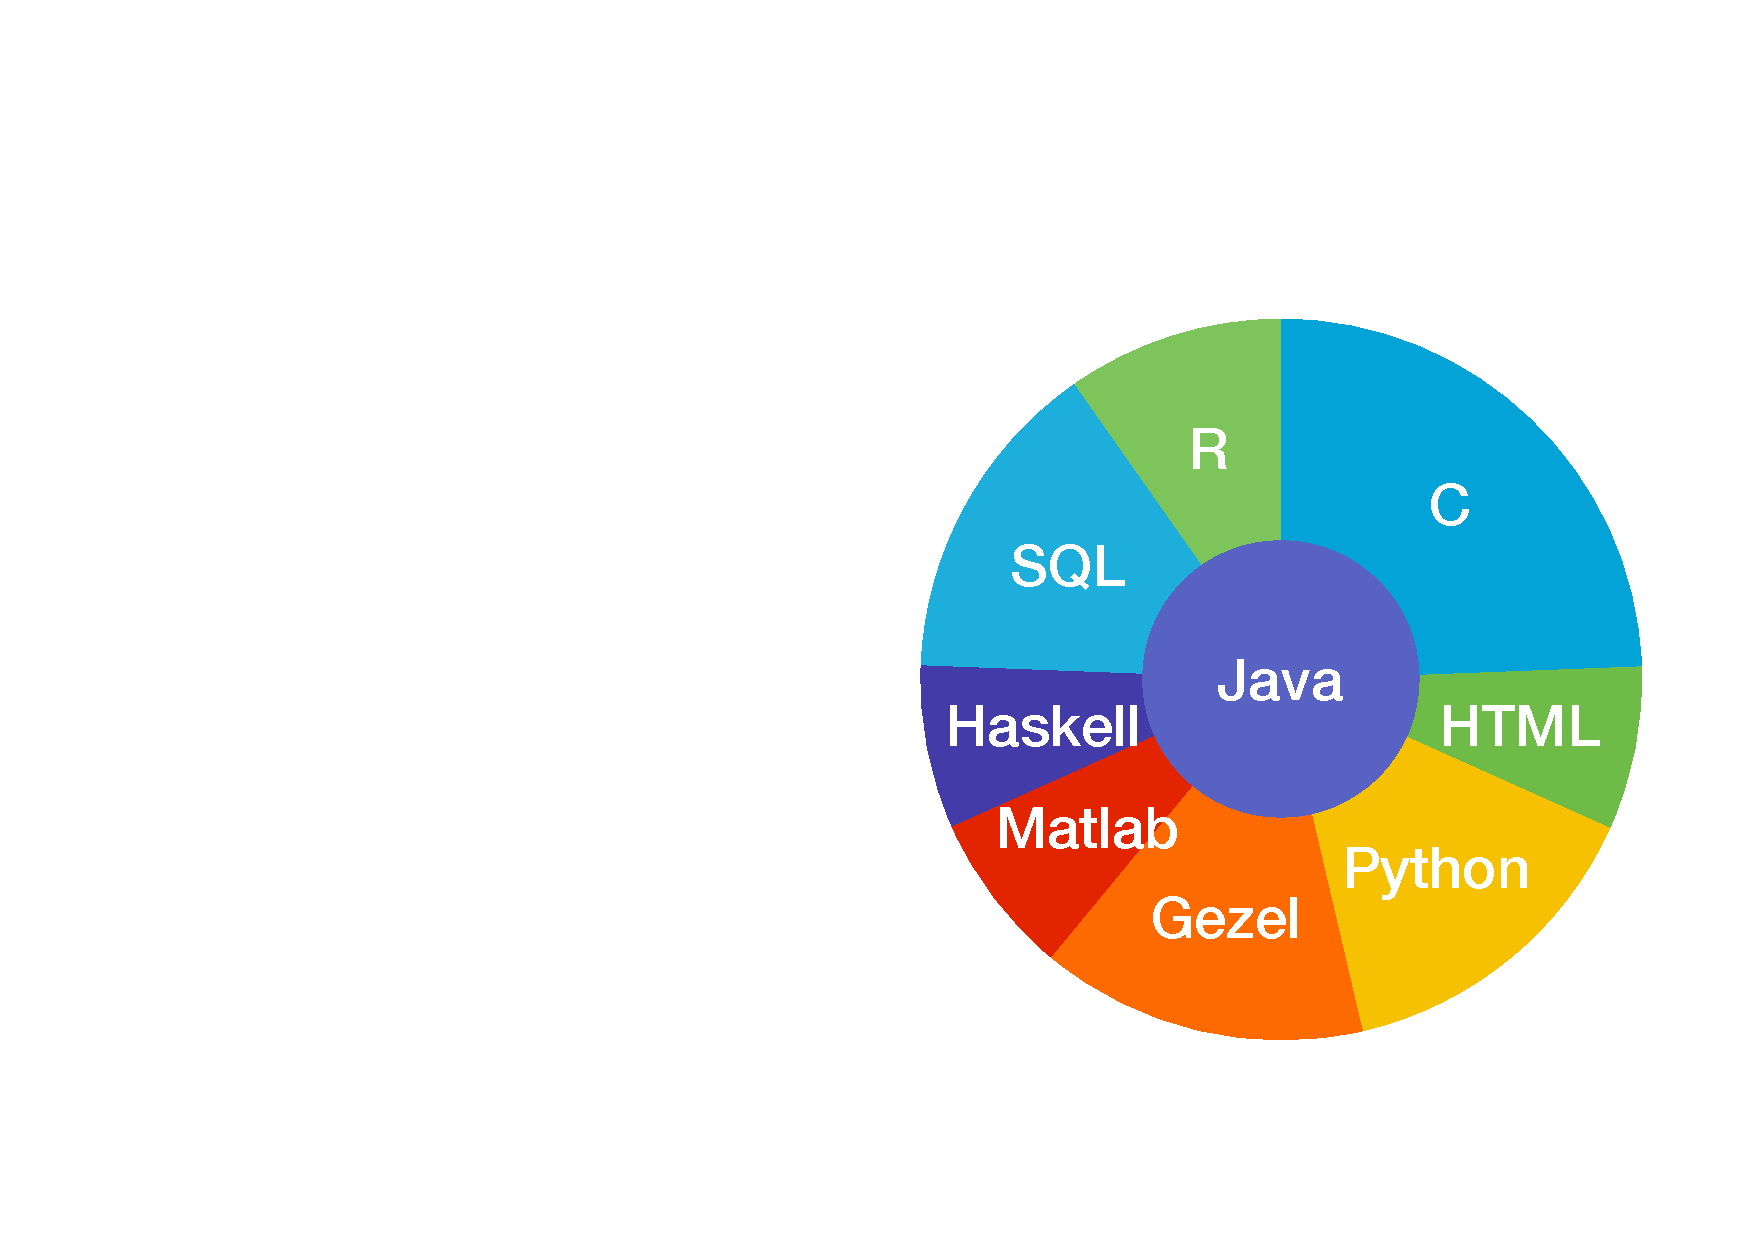
\includegraphics[width=\linewidth]{img/programmeringschart}
    ~
  \section{OS Preference}
    \textbf{MacOS}
\includegraphics[scale=0.40]{img/5stars.png}
    \textbf{Windows}
\includegraphics[scale=0.40]{img/4stars.png}
    \textbf{GNU/Linux}
\includegraphics[scale=0.40]{img/3stars.png}
    ~
  \section{Personal Skills}
    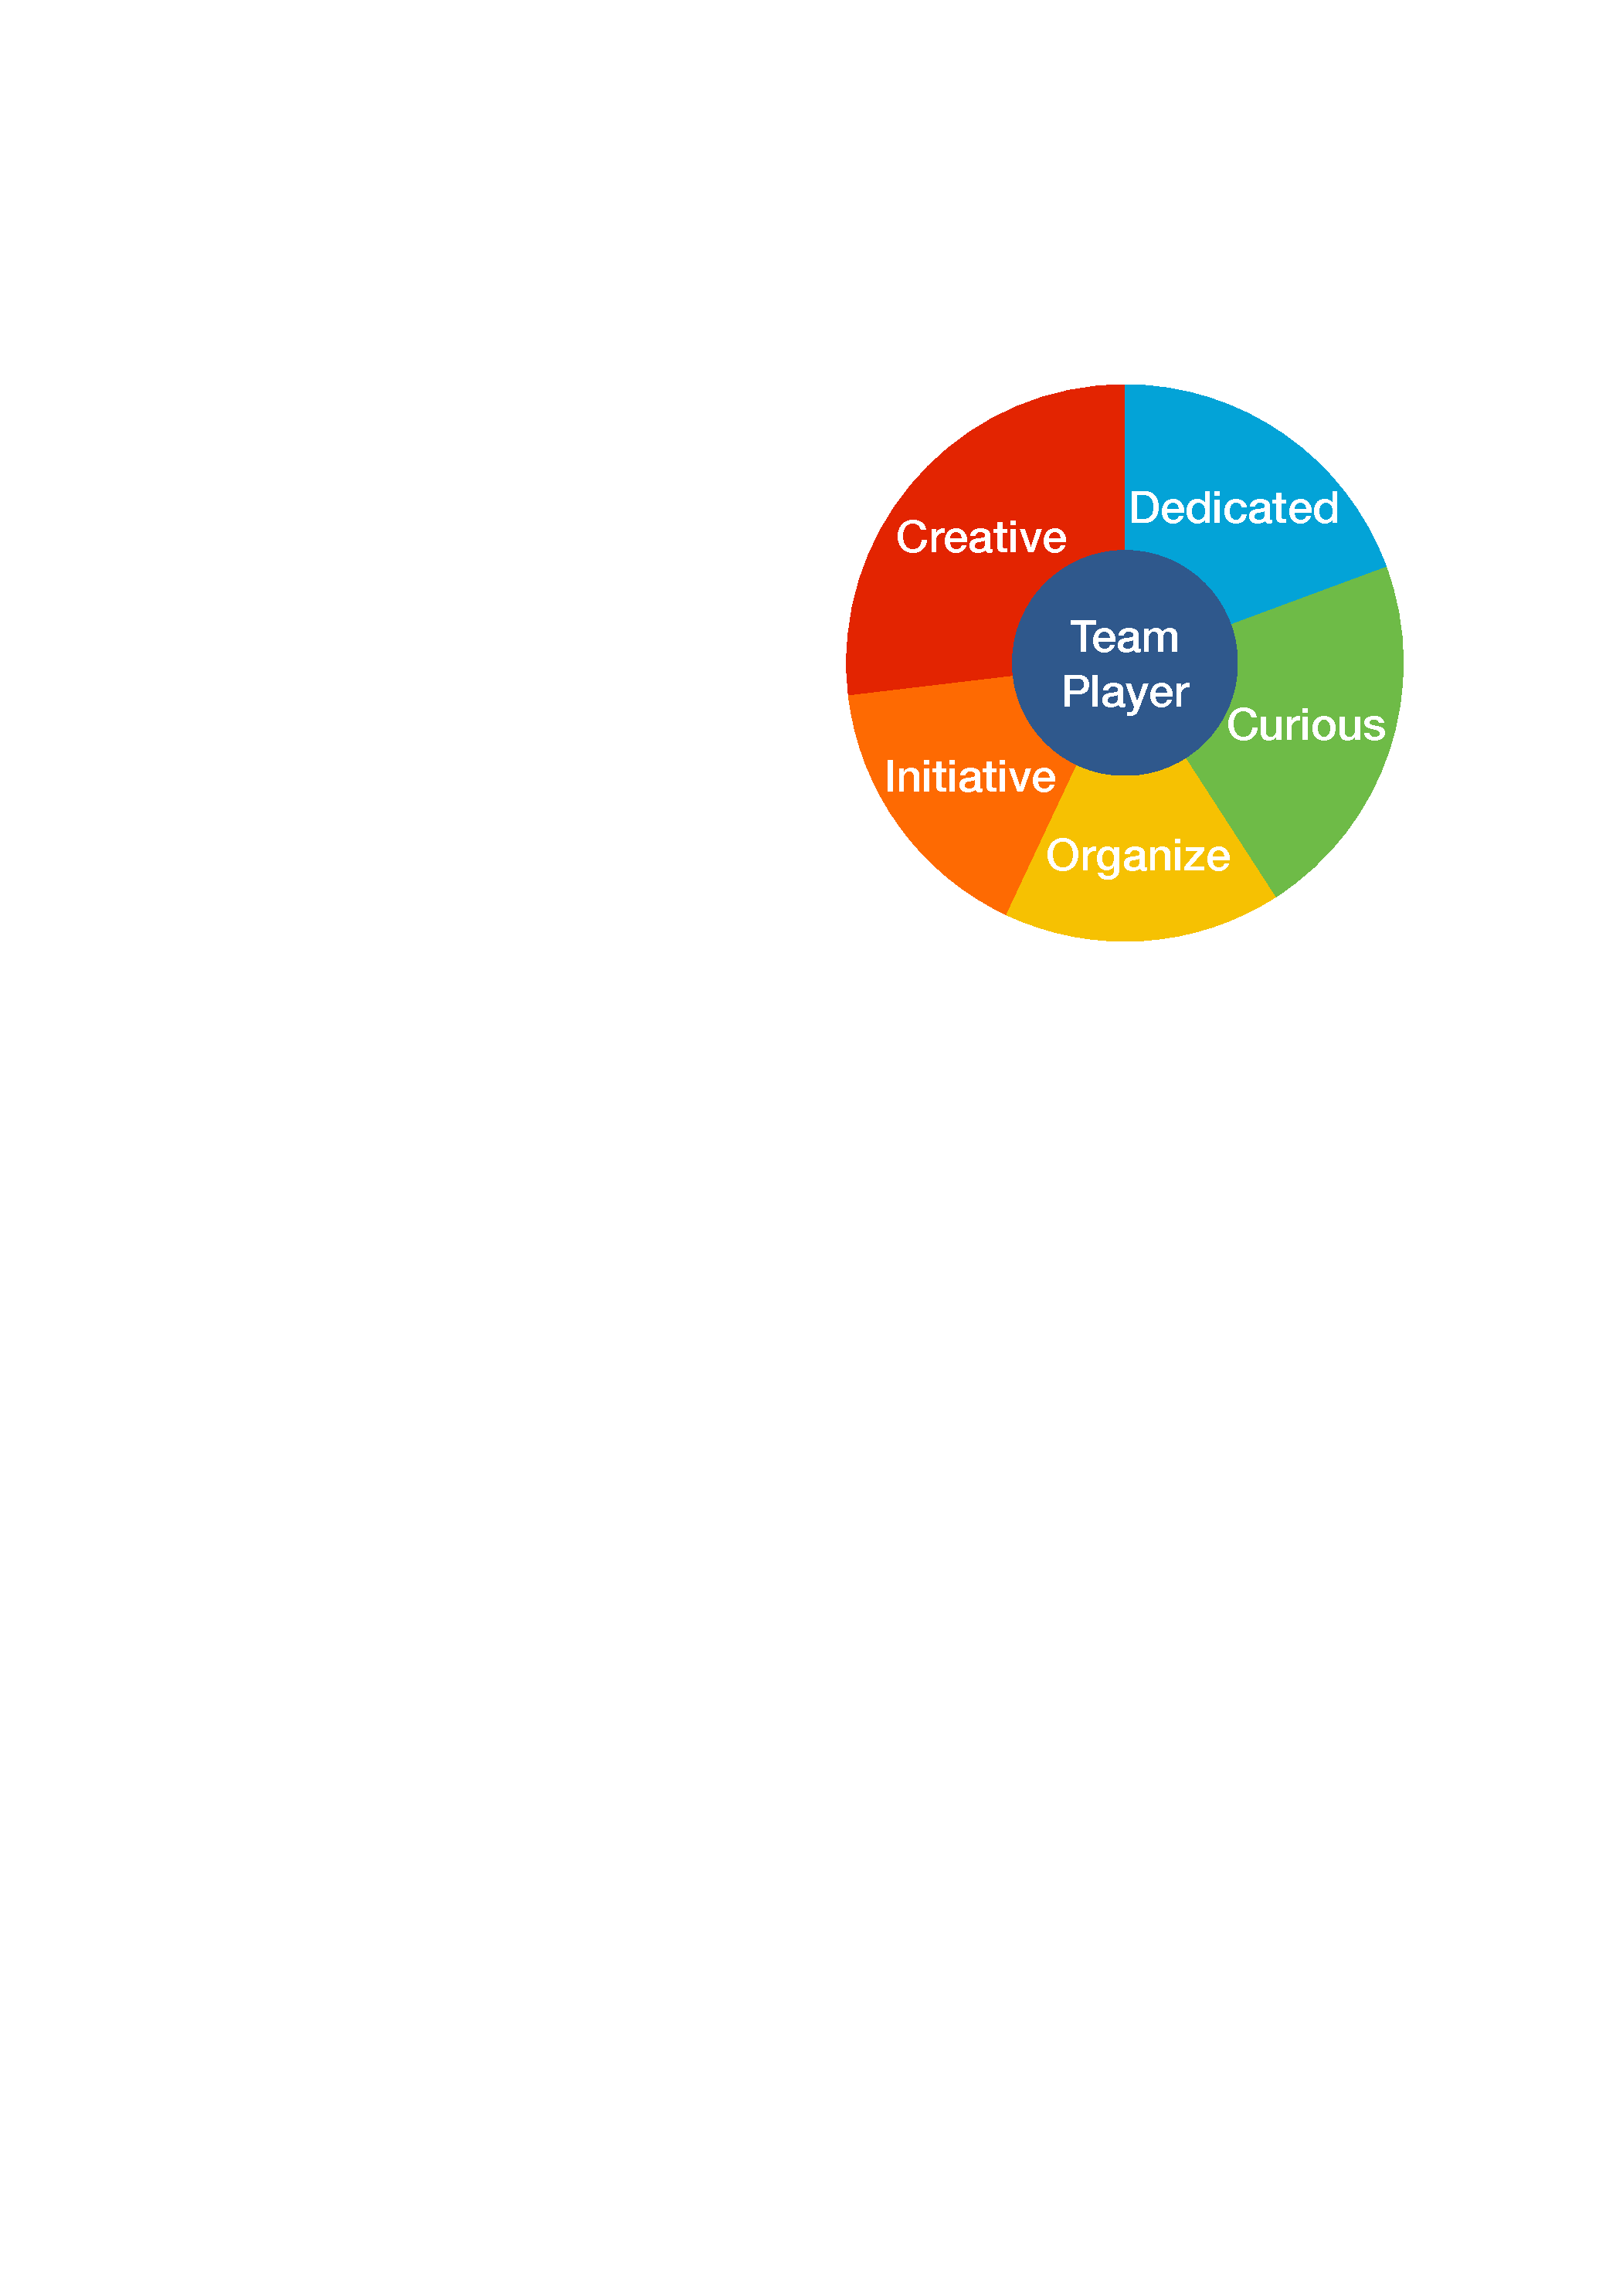
\includegraphics[width=\linewidth]{img/personality.pdf}
    ~
\end{aside}

\section{Education}
\begin{entrylist}
  \entry
    {2016 - now}
    {Bachelor in Computer Science}
    {Technical University of Denmark - DTU}
    {Main subjects: Problem Solving, Systems Architecture, Embedded Systems, Algorithm Efficiency, Model Checking.\\
    \emph{Future subjects: Artificial Intelligence, Machine Learning, Big Data.\\}}
    
  \entry
    {2014 - 2016}
    {Bachelor in Physics and Nanotechnology}
    {Technical University of Denmark - DTU}
    {Main subjects: Mathematics, Mechanical Systems, Electromagnetism, Statistics, Fabrication, Thermodynamics, Programming.\\
    \emph{Change of study: From Physics to Computer Science\\}}
    
  \entry
    {2010 - 2013}
    {Field of Biotechnology}
    {Gymnasium, Slagelse, Denmark}
    {Main subjects: Mathematics, Biotechnology, Physics. \\
    \emph{Exam: Studentereksamen (STX)}}
    
\end{entrylist}


\section{Employment}
\begin{entrylist}
  \entry
    {08/16 - 12/16}
    {Teachers Assistant in Physics1 course}
    {Technical University of Denmark - DTU}
    {Main job: Helping students with the physics course. Assisting teaching the curriculum where needed. Supporting students in need. Correcting assignments. Explain complex systems in an intuitive way.\\}
    
  \entry
    {02/15 - 12/15}
    {Tutor at DTU}
    {Technical University of Denmark - DTU}
    {Main job: Welcome new students. Create a network for new students. Be their tutor in the first semester. Weekly meetings, ensuring everybody is up to date. Organize and manage large social events.
    \\}
    
    
\end{entrylist}


\section{Projects}
\begin{entrylist}
  \entry
    {01/17 - Now}
    {Netbank IBM}
    {Technical University of Denmark - DTU}
    {Main subject: Design and implement a complete local netbank. Using IBM's DB2 database and mainframe. Design pattern following MVC.\\
    \emph{Main languages used: Java, SQL, HTML.}
    \\}
    
  \entry
    {07/16 - 12/16}
    {Embedded ECG scanner}
    {Technical University of Denmark - DTU}
    {Main subject: Design and implement an electrocardiograph. Implementing necessary data filters and program logic in C. Designing the architecture of the central processor unit and co-processor in Gezel. Optimizing the system with respect to speed and low energy usage.\\
    \emph{Main languages used: C, Gezel.}
    \\}
    
  \entry
    {07/16 - 12/16}
    {Checkers Game}
    {Technical University of Denmark - DTU}
    {Main subject: Design and implement a checkers game. Implement necessary game logic. Create a interactive user interface. Design pattern following MVC. \\
    \emph{Main language used: Java.}}
\end{entrylist}
\end{document}
